%% content.tex
%%
\chapter{Erstellen einer Landkarte in D3.js}
\label{ch:map-in-d3js}

\nocite{blocksmercator:2018}

Im Folgenden wird gezeigt, wie man eine einfache Landkarte in D3.js erstellen kann. Dieser Prozess kann in drei logische Abschnitte aufgeteilt werden.

\section{Allgemeines}
\label{sec:map-abstract}

Zu Beginn müssen ein allgemeine Werte wie Breite und Höhe des Bereichs auf dem Bildschirm sowie ein svg-Tag, in den die Landkarte projiziert werden soll, festgelegt werden.

\begin{lstlisting}

var width = 1440;
var height = 750;

var svg = d3.select("body")
        .append("svg")
        .classed("map", true);

var background = svg.append("rect")
        .attr("width", width)
        .attr("height", height)
        .classed("background", true);

\end{lstlisting}

\section{Anlegen von Projektions- und Pfadfunktion}
\label{sec:map-setup}

Danach müssen die in beschriebenen Projektions- und Pfadfunktionen angelegt werden, mithilfe derer dann die Landkarte gezeichnet werden kann.

\begin{lstlisting}

var projection = d3.geoEquirectangular()
        .scale(width / 2 / Math.PI)
        .translate([width / 2, height / 2]);

var path = d3.geoPath()
        .projection(projection);

\end{lstlisting}

\section{Einlesen und Verarbeiten der zu projizierenden Daten}

Zuletzt muss noch die Datei, welche die zu projizierenden Daten repräsentiert, eingelesen und verarbeitet werden.

\begin{lstlisting}

var url = "..."; // URL, die auf die zu verarbeitende Datei verweist

d3.json(url, function(geojson){
    svg.append("path")
            .attr("d", path(geojson));
});

\end{lstlisting}

Die entstehende Landkarte hat dieses Aussehen:

\begin{figure}[H]
    \centering
    
    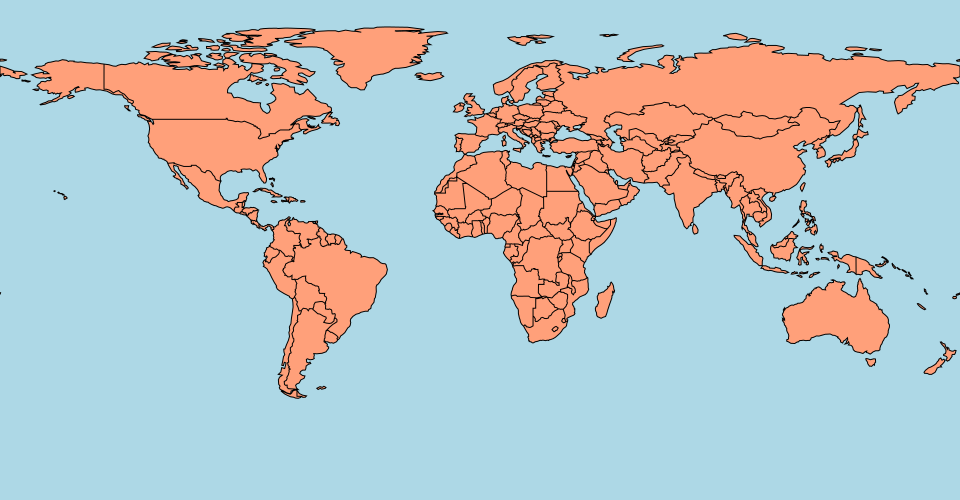
\includegraphics[width=.5\textwidth]{images/mapSinglePath}
    \caption{\glqq Natural Earth\grqq -Projektion}
\end{figure}